Adresářová struktura programu modelu \smod s popisem nejdůležitějších adresářů 
je ukázána na obrázku~\ref{fig:adresare} v příloze~\ref{sec:priloha}. 
Klíčovým adresářem je adresář {\tt bin/}, kde jsou uložené gui plug-iny pro použitím modelu v ArcGis
a dalších GIS softwarech. V adresáři {\tt smoderp2d/} je uložený samotný zdrojová kód modelu. 
Dalším důležitým adresářem je adresář {\tt smoderp2d/providers}, kde jsou uloženy třídy  
pro {\it preprocessing} vstupních dat (v této verzi modelu implementovaný pomocí ArcGIS). 
Jak je vidět na obrázku~\ref{fit:adresare}, v adresáři {\tt smoderp2d/providers} jsou uloženy
třídy pro 2 další GIS softwary. V současné verzi modelu zůstává použití jiných GIS softwaru pouze experimentální. 
V adresáři {\tt tests/data} jsou uložena testovací data. Jedná se o data experimentálního
povodí Nučice, kde katedra KHMKI ČVUT v Praze provádí výzkum srážko-odtokových a erozních procesů
na měřítku malého zemědělského povodí. Do adresáře {\tt tests/data} jsou rovněž
uloženy výsledky testovací úlohy. 

% Důležitými soubory jsou rovněž soubory {\tt src/runoff.py} a {\tt src/time\_step.py}, 
% kde probíhá samotný výpočet. Soubory v adresáři {\tt src/main\_clasess/} obsahují 
% definici datových struktur jednotlivých řešených dějů a skládají dohromady metody 
% k řešení jednotlivých častí odtoku. Tyto metody jsou pak definované v adresáři {\tt src/processes/}. 

Program \smod je napsaný v jazyce Python. Python je často používaný GIS softwary jako skriptovací jazyk a jsou pro něj k dispozici knihovny pro efektivní práci s geodaty\footnote{knihovna {\tt arcpy} pro ArcGIS či knihovny {\tt grass.script} pro GRASS GIS}. Programy či skripty napsané pomocí Python jsou spustitelné v prostředí daných GIS softwarů. Současná verze modelu \smod používá Python 2.7.X, který je kompatibilní s ArcGIS 10.X.

Na obrázku~\ref{fig:flowchart} v příloze~\ref{sec:priloha} je zjednodušený diagram toku programu. Program řeší v každém časovém kroku rovnici~(\ref{eq:bilancnirce}). Pokud je překročena kritická výška a půda se začne vymílat, začne se do celkového  odtoku  započítávat i soustředěný odtok. Bilanční rovnice je rozšířena (\ref{eq:bilancnircerill}). Pokud je řešen i odtok hydrografickou sítí, načítá se celkový přítok $\sum_j^m \acs{oin}_{j,t-1}$ (případně $\sum_k^n \acs{oinrill}_{k,t-1}$) v rovnici~(\ref{eq:bilancnirce})  nebo (\ref{eq:bilancnircerill}) do všech buněk ležících v daném úseku. Odtok je následně řešen Manningovou rovnicí.

Pokud v daném časovém kroku překročí rychlost v jakékoli buňce \acs{CFL} kritérium, dojde ke zmenšení časového kroku a výpočet se v daném kroku opakuje. Pokud je \acs{CFL} kritérium nízké, je možné časový krok zvýšit. To odpovídá kontrole a aktualizaci časového kroku v diagramu na obrázku~\ref{fig:flowchart}. Po dosažení konečného času dojde k uložení výsledných hodnot a ukončení programu. Pravidla \acs{CFL} kritéria jsou popsána v kapitole~\ref{sec:cfl} a implementována v souboru {\tt src/courant.py}.





% 
% \begin{itemize}
% \item main.py
% \item constants.py
% \item rainfall.py
% \item functions.py
% \item runoff.py
% \item data preparation.py
% \end{itemize}
% 

% \textbf{z diplomky:}
% Samotný model je spouštěn je ze souboru main.py, kde podle zvoleného typu výpočtu je importován příslušný soubor. V současnosti se jedná o soubor runoff.py. Na začátku je provedena příprava dat. Jedná se o soubor data preparation.py. Jádrem přípravných prací je vytvořit ze vstupních dat rozsah řešeného území a vytvořit vrstvu směrů přítoků do jednotlivých buněk. V souboru constants.py jsou označeny vstupy. Soubor functions.py shromažďuje funkce, které se v programu opakují, aby je bylo možno znovu snadněji použít. Soubor rainfall.py převede vstupní textový soubor srážkové události na jednotlivé úhrny podle časového kroku modelu. Samotný výpočet probíhá v jádru souboru runoff.py. Pro jednotlivé časové kroky je vypočítáván povrchový odtok. Výpočet probíhá rozdílně na dvou typech buněk. Plošný odtok je počítán v buňkách, kde hladina nepřekročila hladinu kritickou pro soustředění odtoku a rýhový odtok na buňkách, kde tato hranice překročena byla. Výpočet probíhá ve vícerozměrných maticích. Výsledkem jsou rastry, polygonové vrstvy a textové soubory.




% \textbf{doplnit}
% \begin{itemize}
% \item že se vstupy natahují z AG
% \item časový cyklus
% \item plnění matic a jak je to v matici zapsáno
% \item práce s elementama
% \item co si model pamatuje do dalšího kola
% \item testování výpočtu CLF
% \end{itemize}
% 
% \begin{large}
% \textbf{Někde najité texty}
% \end{large}

% Objektově orientované zpracování toku programu umožňuje jednak lepší orientaci v kódu a také lepší běh programu. Jednotlivé procesy jsou ro







\subsection{Programovací jazyk Python} \label{sec:python}
  Python je vysokoúrovňový objektově orientovaný programovací jazyk, který se může využít v~mnoha oblastech vývoje softwaru. Nabízí významnou podporu k~integraci s~ostatními jazyky a~nástroji a~přichází s~mnoha standardními knihovnami. Jeho použití je velice široké od~programů na~zpracování multimedií až~po~zpracování textů. Python je multiplatformní programovací jazyk~\citep{python}. Zajímavým balíčkem jazyka Pyhton je {\tt numpy}~\citep{numpy}. Je to balíček užívaný pro~vědecké výpočty. Umožňuje manipulaci s velkými multi-dimenzionálními poli a disponuje velkou knihovnou matematických funkcí pro~práci s~těmito poli. Pomocí tohoto balíčku bylo v~programu operováno s~naprostou vetšinou polí a~matic. 
  
  Aktuální verze modelu \smod používá Python 2.7. V~současnosti (Prosinec 2017) je nejnovější verze jazyka Python 3.6. Poslední verze vývojové větve Pythonu 2.7 vyšla v~roce 2010.  Podpora Python 2.7 je plánována do jara 2020 (přesné datum zatím není stanoveno). S koncem podpory Python 2.7 končí i implementace této verze v gis softwarech. ArcGIS PRO již podporuje výhradně Python 3. Proto bude docházek k migraci modelu \smod na verzi  Python~3. 

  
  
  
  
  
  
\subsection{CFL podmínka - řešení nestability výpočtu} \label{sec:cfl}
  V předchozích verzích modelu \smod nebyla ošetřena podmínka stability výpočtu, která vychází z řešení časové derivace. Při větších rychlostech toku či nevhodně zvolené délce časového kroku docházelo k nestabilitám v řešení. Program se v takovém případě ukončil a uložil výsledky posledního úspěšně spočítaného časového kroku. 

  V současné verzi programu \smod je tento problém vyřešen Courant-Friedrich-Lewy (\acs{CFL}) podmínkou. Splnění této podmínky zajišťuje konvergenci explicitního řešení pokud platí, že $\acs{CFL} < 1.0$. Z obecné rovnice \acs{CFL} podmínky byla odvozena a upravena podmínka pro účely modelu \smod na následující tvar: \pozn{neni k tomu 0.5601 nejak citace?} 
  \begin{equation}
    \acs{CFL} = \frac{1}{0.5601}\frac{v \acs{dT}}{\acs{dX}} 
    \label{eq:courrovnice}
  \end{equation}
  \begin{tabular}{rrl}
    kde \jj{CFL}{,}
        & $v$ & je rychlost plošného či rýhového toku [$m/s$], \\
        \jj{dT}{\ a}
        \jj{dX}{.}
  \end{tabular}
  
  Po dokončení výpočtu  časového kroku je uložena nejvyšší hodnota \acs{CFL} zjištěná z {\bf plošného odtoku} pomocí vztahu~(\ref{eq:courrovnice}). Poté se tato hodnota porovná s kritickou hodnotou \acs{CFL} a podle pravidel znázorněných v tabulce~\ref{tab:cflsheet} se změní (nebo nezmění) délka časového kroku \acs{dT}. Pokud dojde ke změně \acs{dT} opakuje se výpočet v daném časovém kroku a aktualizovaným \acs{dT}. Do dalšího času se výpočet posune, až když je zaručena stabilita výpočtu. 
  
  \begin{table}[t!]
    \centering
    \caption{Kritéria změny časového kroku vycházející z plošného odtoku}
    \label{tab:cflsheet}
    \begin{tabular}{ccc}
      \hline
        nové  &  $\acs{CFL} < 0.75 \lor 1.0 < \acs{CFL}$ & $ 0.75 \geq \acs{CFL} \geq 1.0 \lor \acs{CFL} = 0.0^*$ \\
        \hline
        \hline
        \acs{dT} &  = $MIN(\frac{0.5601\acs{dX}}{v};\acs{dTmax})$ & = původní \acs{dT}\\
        \hline
%         \multicolumn{3}{l}{{\small \acs{CFL} = 0.0 zpravidla v případně, pokud je rychlost proudění nulová. Potom nelze }}
    \end{tabular}
  \end{table}

  {\bf Soustředěný odtok} v  rýhách je zpravidla řádově rychlejší než plošný odtok. Pokud bychom v tomto případě uplatňovali stejný princip jako u plošného odtoku, časový krok by byl extrémně malý, čímž by se prodlužoval strojový čas výpočtu. K odtoku v rýhách většinou nedochází na celém území, ale pouze v poměrně malém počtu buněk (v poměru k celé ploše výpočetní oblasti). Proto se při výpočtu soustředěného odtoku přistoupilo k lokálnímu krácení časového kroku pouze v buňkách, kde k soustředěnému odtoku dojde. Časový krok výpočtu odtoku v rýhách je dělen celočíselně faktorem označeným jako \acs{ratio}.  \acs{CFL} číslo se proto ukládá zvlášť u plošného a zvlášť u soustředěného odtoku. Ke změně celkového časového kroku plošného odtoku dojde až pokud $\acs{ratio} >= 10$. Časový krok plošného odtoku je pak násoben multiplikátorem \acs{dTmult}, který se po každém překročení kritické \acs{CFL} podmínky zmenší na 90 \% své dosavadní hodnoty. Pokud je \acs{CFL} kritérium příznivé (začíná se zmenšovat), multiplikátor \acs{dTmult} se postupně zvětšuje vždy o 10 \% dokud nedosáhne hodnoty 1. Pravidla pro změna faktoru \acs{ratio} a multiplikátoru \acs{dTmult} jsou shrnuta tabulce~\ref{tab:cflrill}.
  \begin{table}[t!]
    \centering
    \caption{Kritéria změny faktoru \acs{ratio} při dělení časového kroku pří výpočtu rýhového odtoku}
    \label{tab:cflrill}
    {\small
    \begin{tabular}{llll}
      \hline
        nové  &  $\acs{CFL}_{rill} < 0.3 $ & $ 0.5 < \acs{CFL}_{rill}$ & $ 0.3 \geq \acs{CFL}_{rill} \geq 0.5 $ \\
        & & & $\lor \acs{CFL}_{rill} = 0.0 $ \\
        \hline
        \hline
        \acs{ratio} &  = $MAX(\acs{ratio} - 1;1)$ &  = $MIN(\acs{ratio} + 1;9)$ & = původní \acs{ratio}\\
                     &                              &  pro \acs{ratio} = 10  &                            \\
        \acs{dTmult} &  = $MIN((1/0.9)\acs{dTmult};1)$ &  = $0.9\acs{dTmult}$ & = původní \acs{dTmult}\\
        \acs{dT}    &  & \multicolumn{2}{l}{= $\acs{dT}\acs{dTmult}$} \\
        \hline
        
    \end{tabular}
    }
  \end{table}
  
  
  Obrázek \ref{fig:cfl1} a \ref{fig:cfl2} ukazují chování časového kroku v případě, že je řízen plošným (obrázek~\ref{fig:cfl1}) nebo soustředěným odtokem (obrázek~\ref{fig:cfl2}). 
%   
%   
  \begin{figure}[p]
    \centering
    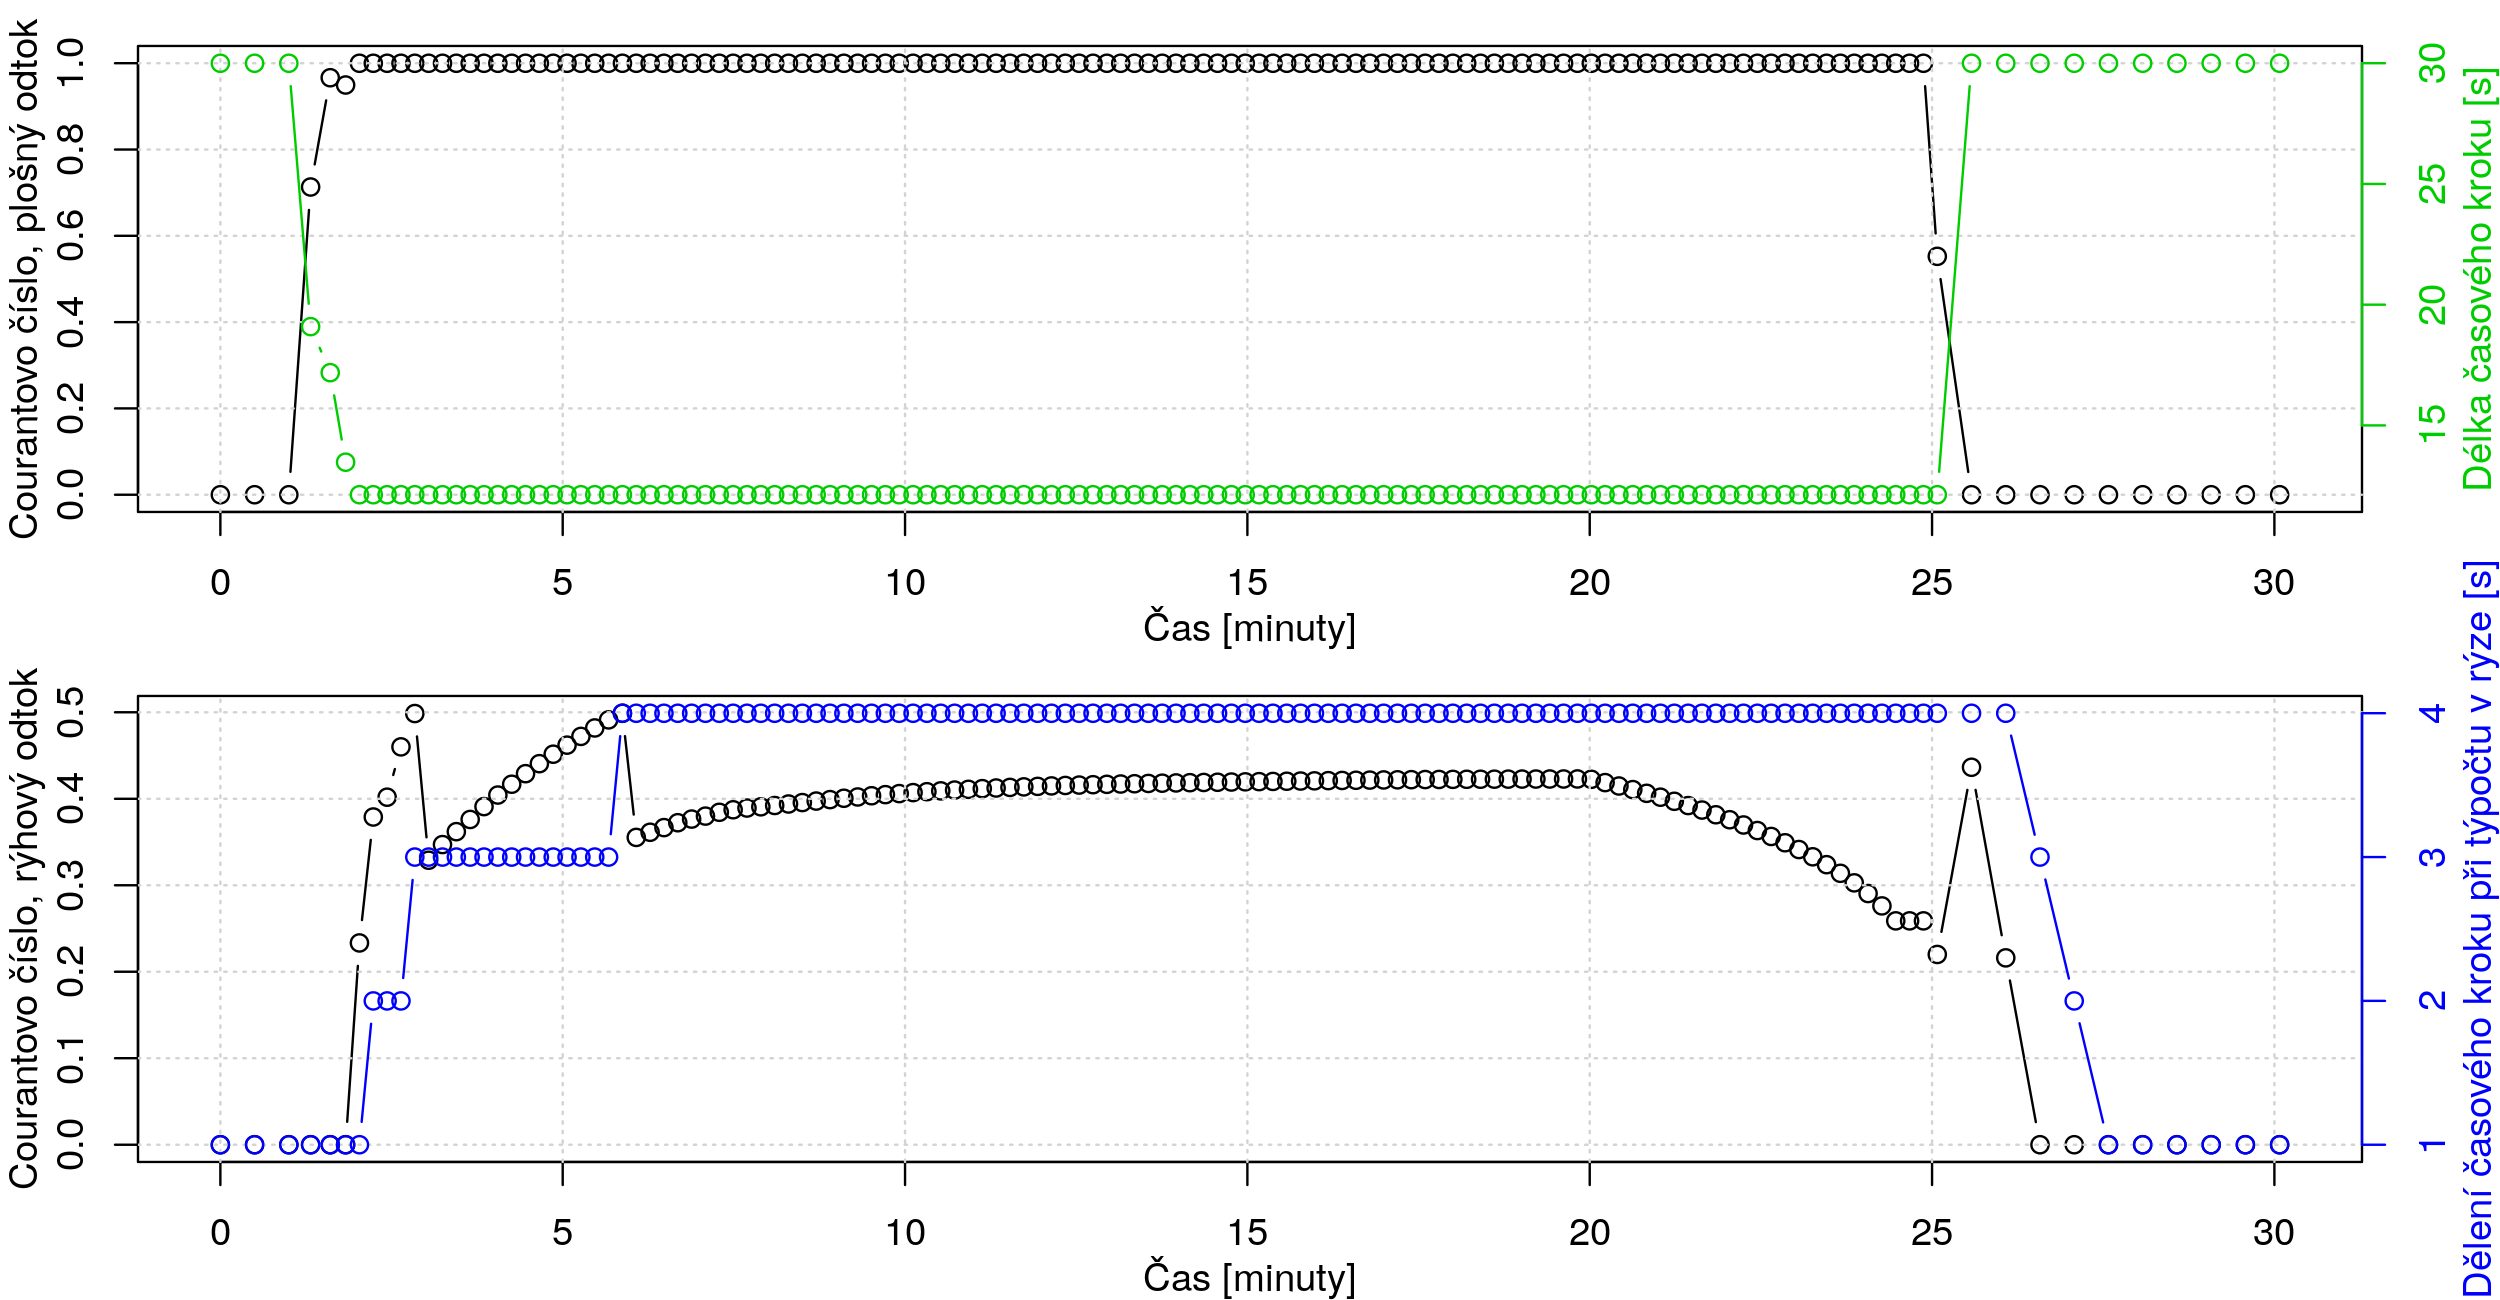
\includegraphics[width=0.8\textwidth]{./img/courantratio.png}
    \caption{Časový krok je řízen rychlostí plošného odtoku. \acs{CFL} rychle stoupne k 1 a začne zkracovat časový krok (horní graf). O pár minut později $\acs{CFL}_{rill}$ stoupne nad 0.5, \acs{ratio} stoupne na 2 (dolní graf) tím začne lokálně dělit časový krok při výpočtu rýhového odtoku. \acs{ratio} na spodním grafu stoupne maximálně na 4 a neovlivní tedy celkový časový krok (na horním grafu). Na obou grafech je vidět, jak se po 25. minutě (kdy v modelu skončila srážková událost) délka časového kroku i \acs{ratio} vrátí na původní hodnoty.}
    \label{fig:cfl1}
  \end{figure}
%   
%   
  \begin{figure}[p]
    \centering
    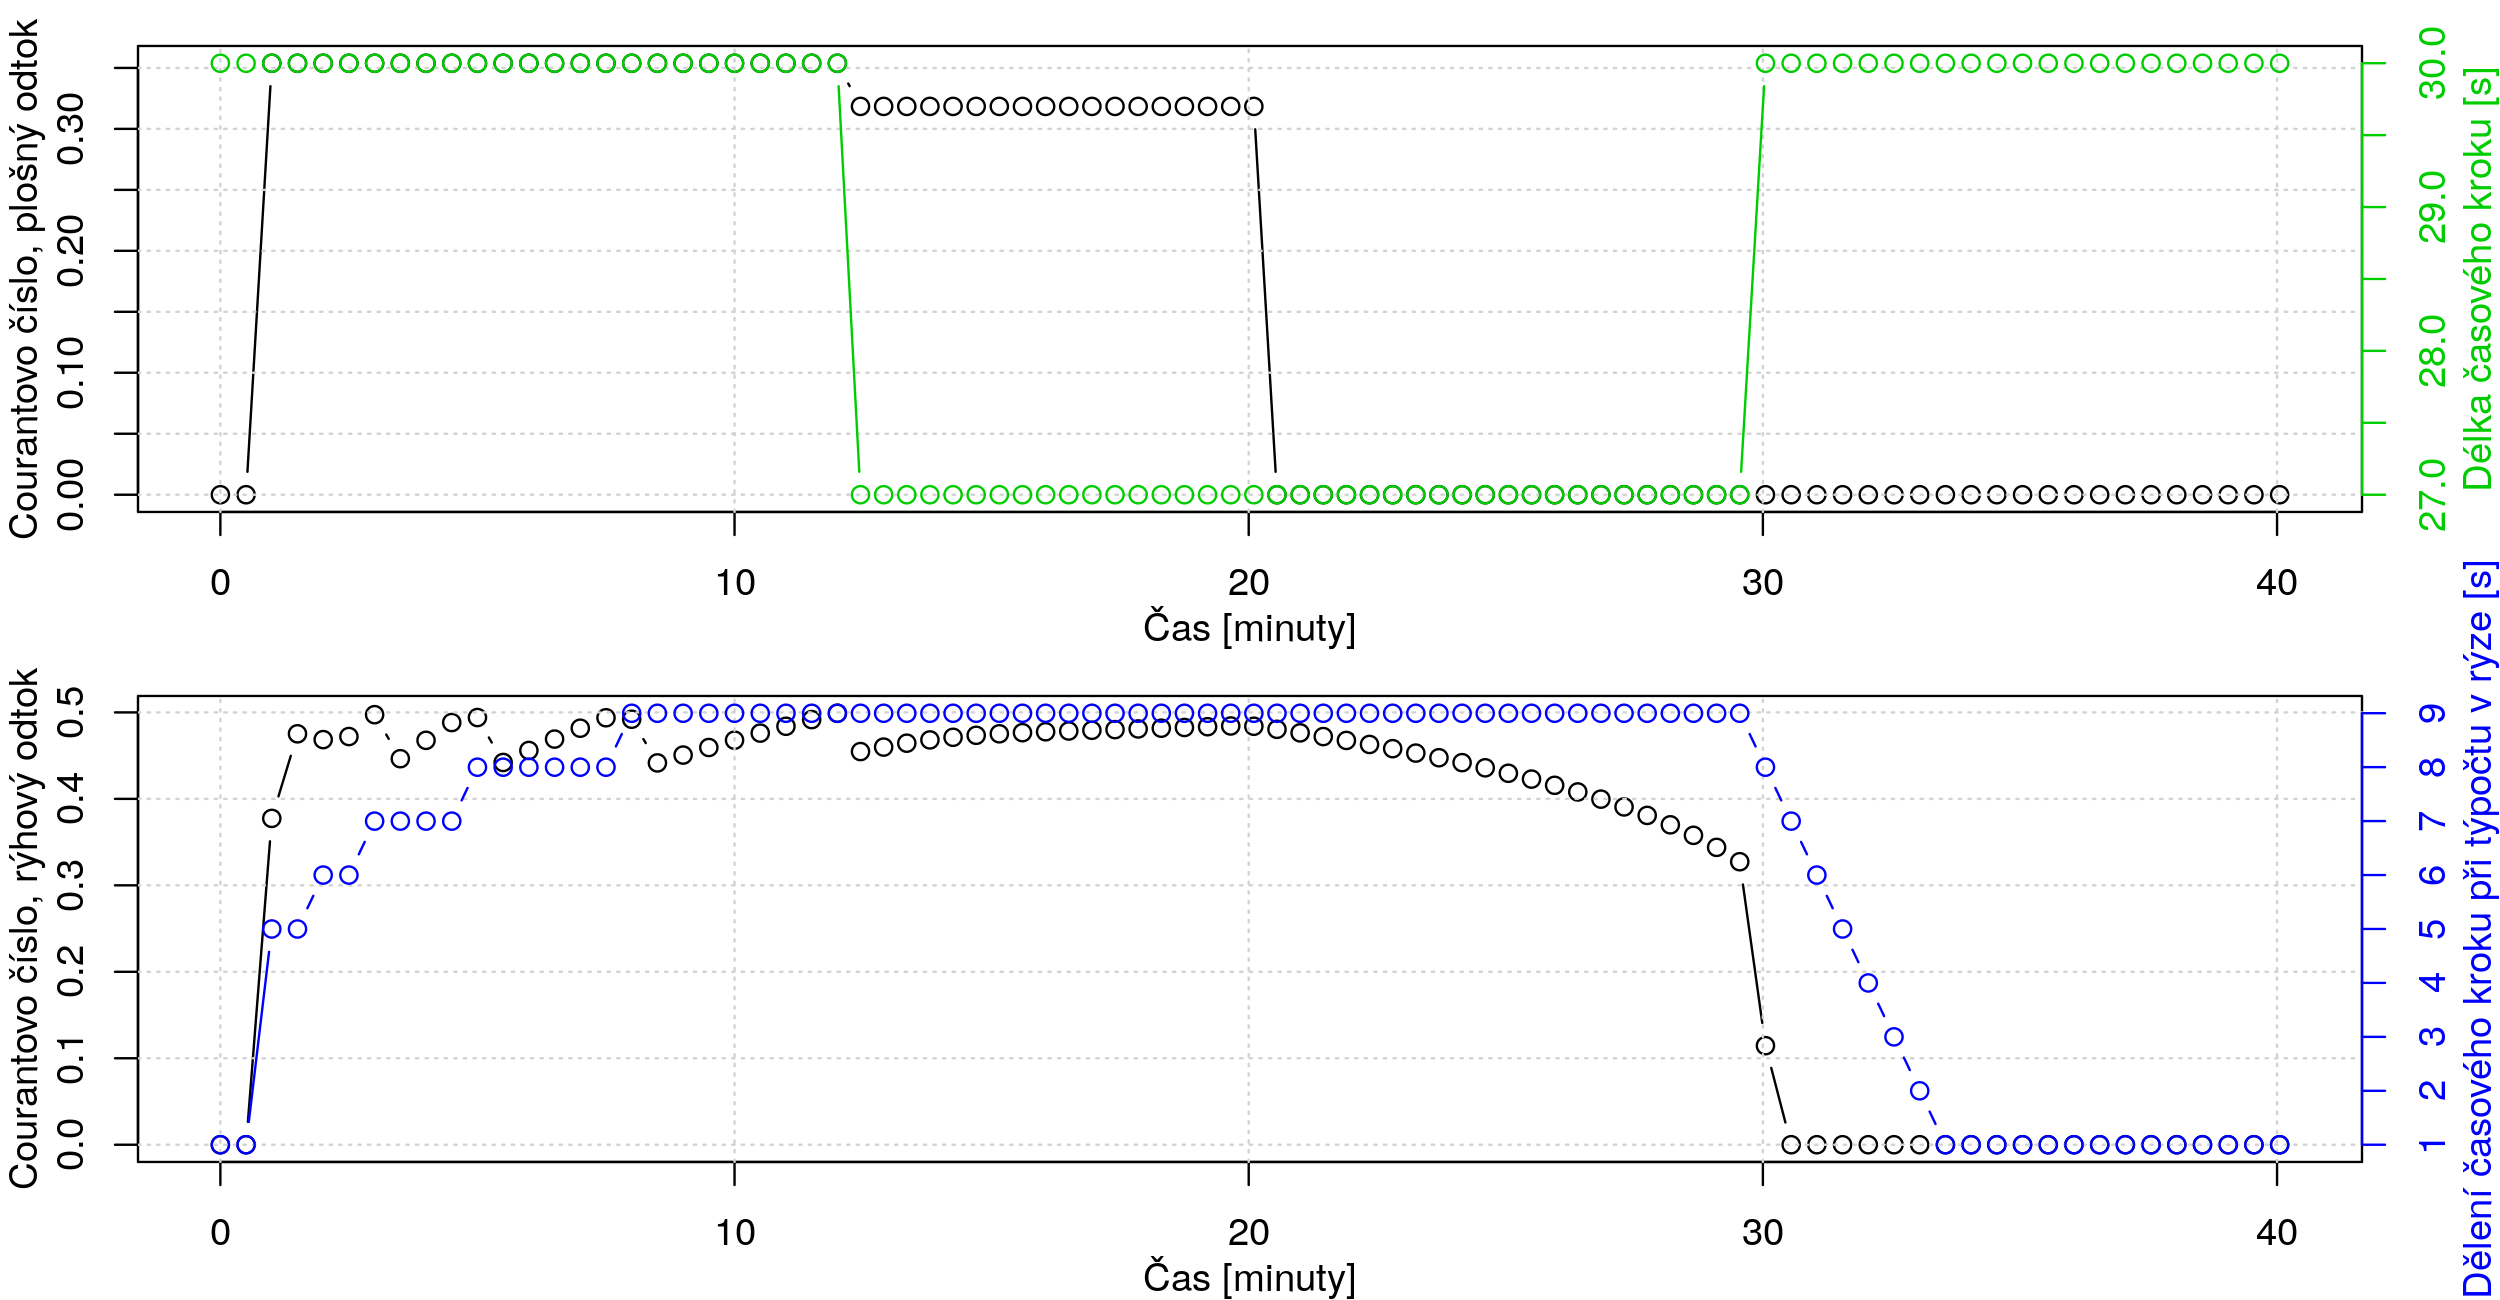
\includegraphics[width=0.8\textwidth]{./img/courantratio2.png}
    \caption{Časový krok je řízen rychlostí rýhového odtoku.  \acs{CFL} plošného odtoku nepřekročí během výpočtu hodnotu cca 0.35 (na horním grafu), proto nemá žádný vliv na velikost časového kroku.  $\acs{CFL}_{rill}$ rychle vystoupí 9 krát nad kritickou hodnotu 0.5 (spodní graf, prvních 10 minut výpočtu). To způsobí nárůst \acs{ratio} na 9, což je maximální povolené dělení lokálního časového kroku při výpočtu rýhového odtoku. Pří dalším překročení hodnot 0.3 (cca 12. minuta na dolním grafu) dojde ke zmenšení celkového časového kroku na 90 \% původní hodnoty (horní graf). Na obou grafech je vidět jak se po 20. minutě (kdy v modelu skončila srážková událost) délka časového kroku i \acs{ratio} vrátí na původní hodnoty.}
    \label{fig:cfl2}
  \end{figure}
  

% Hlavní myšlenkou řešení nestability výpočtu je zmenšení časového kroku při náznaku, že by mohlo dojít k přetečení. Pro každý časový krok je podle rovnice \ref{courrovnice} vypočteno v každé buňce Courantovo číslo $C$. Dále je určeno maximum Courantova čísla ve všech buňkách v časovém kroku. Toto číslo je zásádní, jelikož podle něj se porovnává, zda je situace potencionálně nebezpečná a bude potřeba zmenšit časový krok. Na změnu časového kroku byla použita funkce pojmenovaná $courant$:

% Dochází k porovnání, zda se Courant pohybuje v rozmezí hodnot 0.8 a 1.0. Pokud je hodnota vyšší, je zmenšen časový krok  a pokud je hodnota nižší, časový krok se zvýší. Nikdy však nemůže být výšší než původní časový krok zadaný. Testování probíhalo tak, aby podmínka zmenšila co možná nejméně časový krok a při tom nedošlo k numerické nestabilitě v kroku následujícím. Velikost časového kroku $\Delta t$ zásadně ovlivňuje dobu běhu celého modelu. Čím více se zmenší časový krok, tím déle trvá modelu než doběhne do požadové časové hodnoty a ukončí se. V současné verzi je největším problémem fakt, že při větších průtocích na větším území dojde brzy ke zmenšení $\Delta t$ na velmi nízkou hodnotu, např. 0.01 minuty a tím se úměrně zvyšuje časová náročnost výpočtů.




